\section{Evaluation Design}
\label{sec:experiments}

We evaluate persona datasets along two complementary axes---\emph{forward simulation} (given personas, predict behaviors) and \emph{inverse simulation} (given items, recover personas)---across four grounded evaluation regimes.
Each regime targets a distinct behavioral domain that existing survey-only benchmarks leave untested.
Table~\ref{tab:eval-overview} summarizes the regimes, their granularity, data sources, and the dimension of persona quality each primarily evaluates.

\begin{table*}[t]
\centering
\caption{Overview of the four evaluation regimes. \textbf{Direction}: forward (F) or inverse (I). \textbf{Granularity}: individual, subgroup, or group. \textbf{Primary dimension}: whether the regime primarily stresses \emph{depth} or \emph{coverage} of the persona dataset.}
\label{tab:eval-overview}
\small
\begin{tabular}{@{}llllll@{}}
\toprule
\textbf{Regime} & \textbf{Direction} & \textbf{Granularity} & \textbf{Data Source} & \textbf{Primary Dim.} & \textbf{Key Metric} \\
\midrule
Movie Preferences & F & Subgroup & MovieLens 1M & Coverage + Depth & NDCG, Hit Rate \\
Amazon ICP & I & Individual $\to$ Item & Amazon Reviews 2023 & Depth & KL / JS, Retrieval P/R \\
Reddit Polls & F & Group & Reddit r/polls, Decide-for-me & Coverage & Dist.\ calibration \\
Search Trends & F & Group (locale) & Google Trends, Ahrefs & Coverage & Rank corr., KL div. \\
\bottomrule
\end{tabular}
\end{table*}

\paragraph{Shared evaluation protocol.}
The overarching protocol is shared across all forward-simulation regimes: (1)~align the persona dataset to the target population's demographic distribution, (2)~select task-relevant persona attributes, (3)~prompt an LLM conditioned on each persona to produce a behavioral prediction (rating, ranking, vote, or interest score), and (4)~aggregate persona-level predictions and compare against ground truth.
Alignment strategies and metrics will vary by regime and are to be determined during implementation; we aim to keep the simulation prompt format and aggregation strategy as consistent as possible across regimes to enable cross-regime comparison.
Below we detail the design, rationale, and outstanding assumptions and questions for each regime.


%% ========================================================================
%% REGIME 1: MOVIES (MovieLens 1M)
%% ========================================================================
\subsection{Regime 1: Movie Preferences (MovieLens 1M)}
\label{sec:eval-movies}

\paragraph{Why MovieLens 1M.}
We use MovieLens~1M~\cite{harper2015movielens}, the largest MovieLens release that includes user demographics and one of the most widely used benchmarks in personalization and recommender systems research.
Later releases (10M, 20M, 25M) dropped demographic fields, retaining only anonymized user IDs and ratings.
ML-1M provides the unique combination of scale, rating density, and per-user demographic labels needed for subgroup-level evaluation of persona-conditioned simulation.

\paragraph{Dataset summary.}
ML-1M contains 1,000,209 ratings of 3{,}883 movies by 6{,}040 users who joined MovieLens in 2000, with self-reported demographics collected at registration.
We verified referential integrity: every rating maps to a valid user and movie ID, with zero orphan records.
The dataset has a sparsity of 95.74\% (users rate fewer than 5\% of available movies).
Ratings span April~26, 2000 to February~28, 2003, with a mean rating of 3.582 ($\sigma=1.117$).
Per-user rating counts range from 20 to 2{,}314 (mean~166, median~96), providing substantial per-user signal.
Figure~\ref{fig:ml1m-rating-dist} shows the overall rating distribution; Figure~\ref{fig:ml1m-demographics} summarizes user demographics.

\begin{figure}[t]
    \centering
    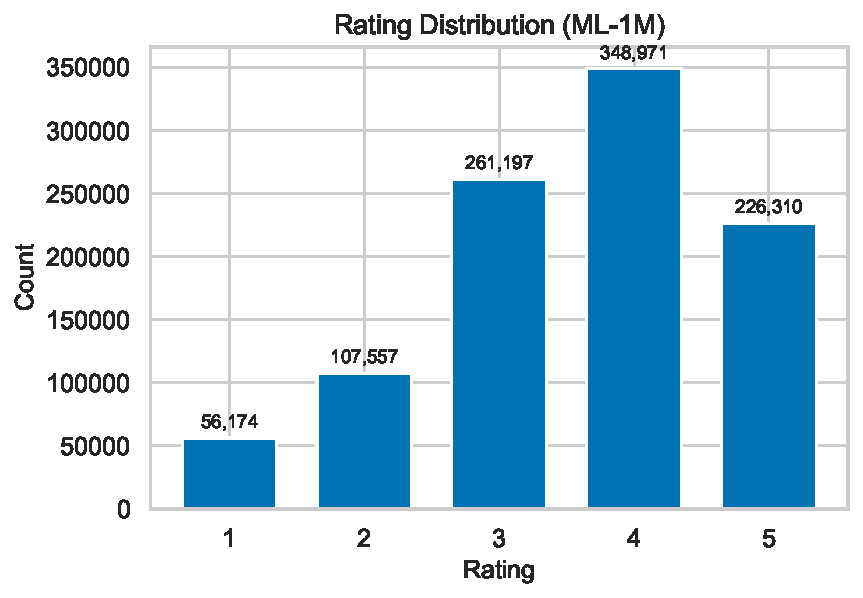
\includegraphics[width=\columnwidth]{images/ml1m_rating_distribution.pdf}
    \caption{Rating distribution in ML-1M. The distribution is left-skewed: ratings of 4 dominate (348{,}971), followed by 3 (261{,}197), 5 (226{,}310), 2 (107{,}557), and 1 (56{,}174). Users rate positively overall (mean 3.58).}
    \label{fig:ml1m-rating-dist}
\end{figure}

\begin{figure*}[t]
    \centering
    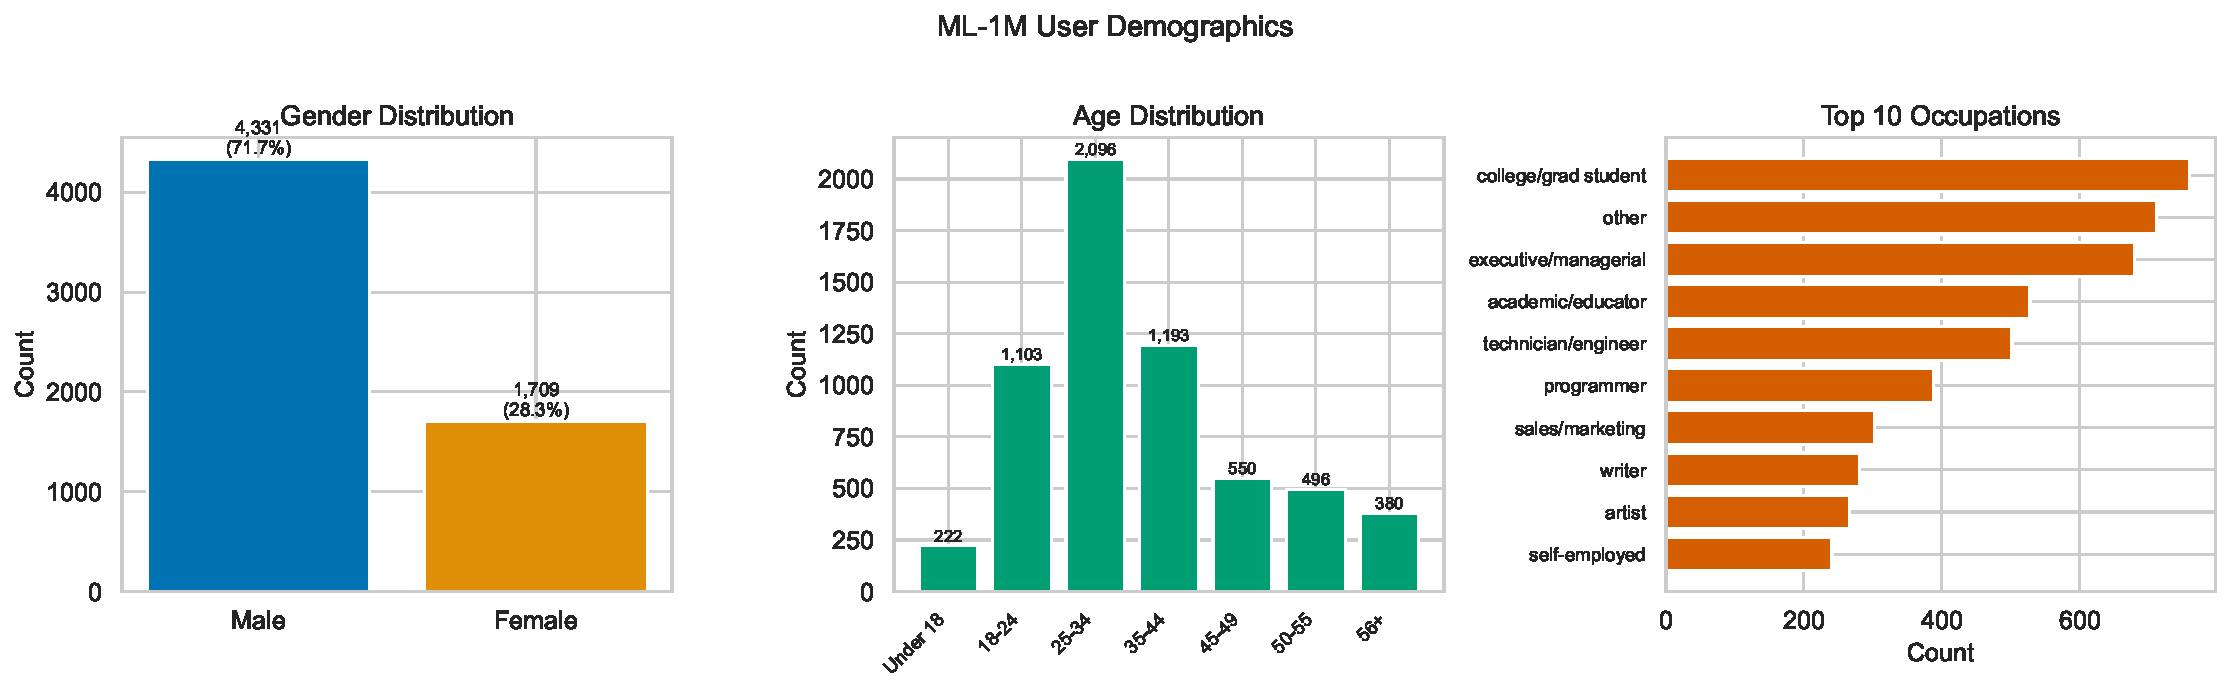
\includegraphics[width=\textwidth]{images/ml1m_demographics.pdf}
    \caption{ML-1M user demographics. \textbf{Left:} Gender split is 71.7\% male / 28.3\% female. \textbf{Center:} The 25--34 age bracket dominates (34.7\%), followed by 18--24 (18.3\%). Users under 18 and over 55 are rare. \textbf{Right:} The top occupation is ``college/grad student'' (12.6\%), followed by ``other'' (11.8\%) and ``executive/managerial'' (11.2\%). The rarest occupation is ``farmer'' (0.3\%, 17 users).}
    \label{fig:ml1m-demographics}
\end{figure*}

\paragraph{Available demographic schema.}
Each ML-1M user record contains four fields:
\begin{itemize}
    \item \textbf{Gender}: binary (M/F).
    \item \textbf{Age}: one of seven coded ranges---Under~18, 18--24, 25--34, 35--44, 45--49, 50--55, 56+.
    \item \textbf{Occupation}: one of 21 categories---academic/educator, artist, clerical/admin, college/grad student, customer service, doctor/health care, executive/managerial, farmer, homemaker, K-12 student, lawyer, programmer, retired, sales/marketing, scientist, self-employed, technician/engineer, tradesman/craftsman, unemployed, writer, other/not specified.
    \item \textbf{ZIP code}: U.S.\ 5-digit ZIP.
\end{itemize}
Ratings are on a whole-star 1--5 scale, each timestamped at second-level resolution.
Every user has at least 20 ratings.
Each movie record contains a title (with release year) and one or more of 18 genres: Action, Adventure, Animation, Children's, Comedy, Crime, Documentary, Drama, Fantasy, Film-Noir, Horror, Musical, Mystery, Romance, Sci-Fi, Thriller, War, Western.

\paragraph{Design.}
We construct the evaluation as a subgroup-level forward simulation task: given a persona matched to a demographic cell in the ML-1M user base, predict the rating distribution or ranked preference list for a held-out set of movies.

\medskip\noindent\textbf{Data preparation pipeline:}
\begin{enumerate}
    \item \textbf{Load and validate.} Parse \texttt{users.dat}, \texttt{ratings.dat}, and \texttt{movies.dat} (all \texttt{::}-delimited). Validate user~ID referential integrity (every rating maps to a known user and movie). Drop the small number of MovieIDs that correspond to duplicate/test entries (noted in the README).
    \item \textbf{Temporal split.} Sort ratings by timestamp. Define a per-user split such that the last $p\%$ of each user's ratings (chronologically) form the test set and the remainder form the observation set. Default $p = 20$; since every user has $\geq 20$ ratings, each contributes both history and held-out items.
    \item \textbf{Subgroup and stratification design.} Our EDA reveals that the full Gender$\times$Age$\times$Occupation space yields 294 possible cells, of which 241 are non-empty and only 82 have $\geq$20 users. We adopt Gender$\times$Age as the primary stratification (14 cells, minimum cell size 78, mean 431), using Occupation as a secondary axis restricted to the 8 most common occupations. Figure~\ref{fig:ml1m-cell-sizes} shows the cell-size distribution; Appendix~\ref{app:ml1m-eda} provides the full cross-tabulation.
\end{enumerate}

\begin{figure}[t]
    \centering
    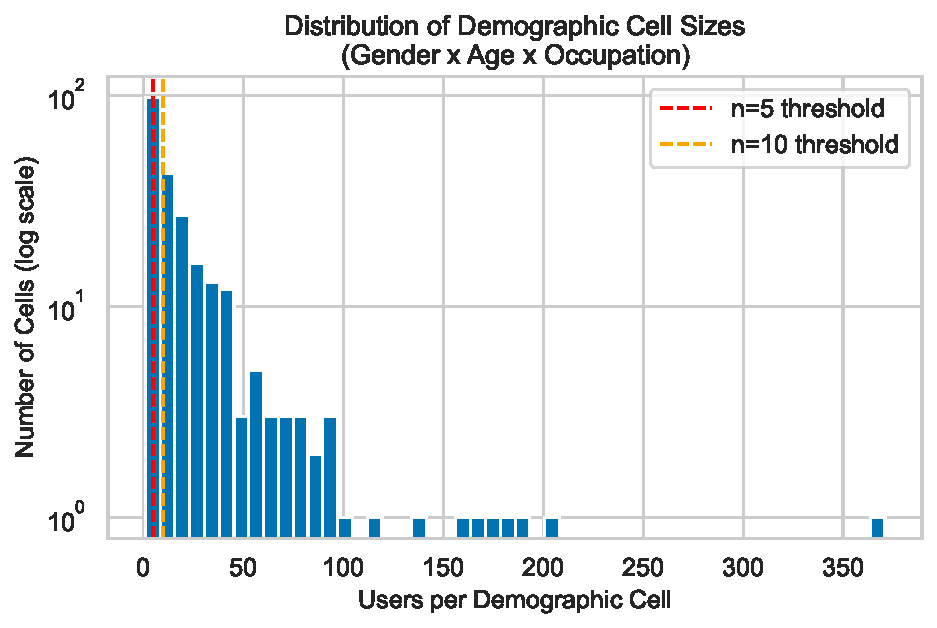
\includegraphics[width=\columnwidth]{images/ml1m_cell_size_distribution.pdf}
    \caption{Distribution of demographic cell sizes (Gender$\times$Age$\times$Occupation). Of 294 possible cells, 53 are empty and 79 have $\leq$5 users (red dashed line). Only 30 cells exceed 50 users. The long tail of sparse cells motivates using Gender$\times$Age (14 well-populated cells) as primary stratification.}
    \label{fig:ml1m-cell-sizes}
\end{figure}

\paragraph{Rationale.}
Movie preferences are among the most expressive dimensions of human identity that survey benchmarks entirely ignore.
A 25-year-old programmer who rates \emph{The Matrix} 5 stars and \emph{Titanic} 2 stars is behaviorally distinct from one who rates both 4 stars, yet census-level personas collapse them.
This regime directly tests whether persona depth---interests, tastes, lifestyle markers---translates into predictive power for consumption behaviors.
The availability of exact demographics per user enables subgroup-level analysis: we can measure whether simulation errors are uniform or systematically worse for underrepresented demographic cells (e.g., older women, farmers, K-12 students).

The choice of ML-1M is deliberate: per-user demographic labels are the critical feature for our evaluation, and ML-1M is the largest MovieLens release that provides them.
The dataset's modest size (${\sim}6$K users) is offset by the density of ratings per user ($\geq 20$), which provides a strong per-user ground truth signal.

\paragraph{Assumptions (verified via EDA).}
\begin{itemize}
    \item \textbf{Self-reported demographics.} Collected at registration (circa 2000) and unverified. Age ranges are coarse but sufficient for subgroup construction; our Gender$\times$Age stratification yields 14 cells with a minimum of 78 users.
    \item \textbf{Rating sincerity.} The left-skewed distribution (mean 3.58, mode 4) is consistent with intrinsically motivated ratings in a recommender system. No evidence of degenerate response patterns (e.g., all-5 or all-1 raters).
    \item \textbf{Binary gender.} ML-1M encodes gender as M/F only (71.7\%/28.3\%), which does not reflect current demographic understanding. This is a limitation of the dataset.
    \item \textbf{Temporal window.} Ratings span April 2000 to February 2003 (35 months). The movie catalog skews pre-2003; the top-rated films (\emph{American Beauty}, \emph{Star Wars} trilogy, \emph{The Matrix}) are thoroughly represented in LLM training data.
\end{itemize}

\paragraph{Questions resolved by data profiling.}
\begin{itemize}
    \item \textbf{Subgroup sparsity (resolved).} Of 294 possible Gender$\times$Age$\times$Occupation cells, 53 are empty and 27 contain exactly one user. Rare cells include ``Female Farmer 35--44'' (1 user) and ``Male Homemaker 18--24'' (1 user). \textbf{Decision:} use Gender$\times$Age (14 cells, all $\geq$78 users) as primary stratification; add Occupation only for the top 8 occupations with a minimum cell size of 20.
    \item \textbf{Popularity bias (quantified).} The Gini coefficient is 0.634, indicating substantial concentration: the top 20\% of movies (741 films) account for 65.2\% of all ratings, while 446 movies (12\%) have fewer than 10 ratings. The most-rated film (\emph{American Beauty}) has 3{,}428 ratings. \textbf{Decision:} include a popularity-debiased evaluation restricted to long-tail movies (bottom 80\% by rating count) to isolate persona contribution from popularity shortcuts. See Figure~\ref{fig:ml1m-popularity}.
    \item \textbf{Within- vs.\ between-demographic variance (quantified).} Demographics explain remarkably little of total rating variance: Gender alone accounts for 0.039\%, Age for 0.376\%, Occupation for 0.268\%, and the full Gender$\times$Age$\times$Occupation cell for only 1.56\% ($\eta^2 = 0.0156$). \textbf{Implication:} within-demographic variance overwhelmingly dominates. This directly motivates persona-level (not just demographic-level) simulation and suggests the evaluation should focus on within-cell differentiation. A demographic-only baseline should perform only marginally above random within cells.
    \item \textbf{Individual vs.\ subgroup evaluation (resolved).} With a 20\% temporal split, every user contributes at least 4 test items (mean 32.7, median 19). This supports individual-level evaluation in addition to subgroup aggregation. \textbf{Decision:} report both individual-level metrics (per-user NDCG) and subgroup-level metrics (aggregated across cells).
    \item \textbf{Genre structure.} Drama (1{,}603 movies) and Comedy (1{,}200) dominate; Film-Noir (44) and Western (68) are rare. Genre preferences differ meaningfully across demographics: older users rate Film-Noir, War, and Documentary significantly higher; younger users favor Sci-Fi, Horror, and Animation. Gender gaps are largest for Horror and Film-Noir (male-preferred) and Romance and Musical (female-preferred). See Appendix~\ref{app:ml1m-eda} for full genre$\times$demographic breakdowns.
\end{itemize}

\begin{figure}[t]
    \centering
    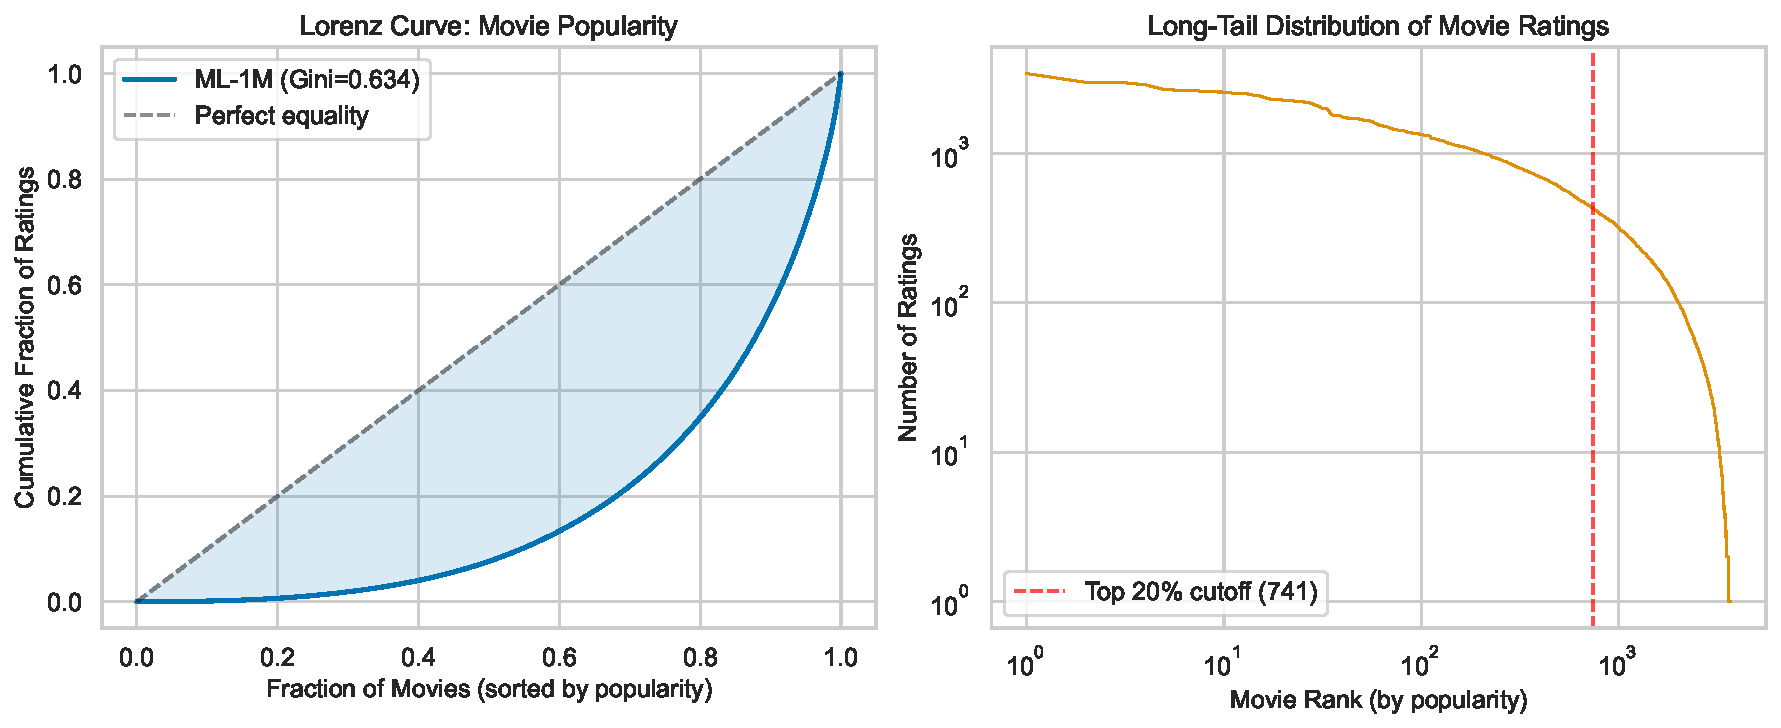
\includegraphics[width=\columnwidth]{images/ml1m_popularity_bias.pdf}
    \caption{\textbf{Left:} Lorenz curve for movie popularity (Gini = 0.634). The bottom 60\% of movies account for only ${\sim}$15\% of ratings. \textbf{Right:} Long-tail distribution on log-log scale; the red dashed line marks the top-20\% cutoff.}
    \label{fig:ml1m-popularity}
\end{figure}

\paragraph{Open questions (requiring further investigation).}
\begin{itemize}
    \item \textbf{LLM memorization floor.} Pre-2003 movies are thoroughly represented in LLM training data. A zero-shot baseline (no persona conditioning) is needed to quantify how much the LLM can predict from movie knowledge alone.
    \item \textbf{User ID overlap with ML-25M.} The ML-25M README states that user IDs are not consistent across releases, so cross-referencing is not reliable without additional verification. We proceed with ML-1M only.
    \item \textbf{Movie metadata enrichment.} ML-1M provides only title, release year, and genre codes. The MovieLens Tag Genome provides tag relevance scores and may serve as a license-compatible enrichment source. Alternatively, title+year can key into TMDb for synopses.
    \item \textbf{Persona attribute saturation.} How many attributes beyond demographics improve prediction? This is an empirical question to address during the simulation experiments.
    \item \textbf{Temporal gap.} The 2000-era temporal window means personas from 2023 Reddit data may not perfectly align with year-2000 tastes. The evaluation tests the LLM's ability to bridge this gap, which is informative regardless of the direction of the result.
\end{itemize}


%% ========================================================================
%% REGIME 2: AMAZON ICP
%% ========================================================================
\subsection{Regime 2: Ideal Customer Profiling via Amazon Reviews}
\label{sec:eval-icp}

\paragraph{Design.}
We construct the first grounded ICP evaluation benchmark from the Amazon Reviews 2023 dataset~\cite{hou2024bridging}, released by the McAuley Lab (UCSD).
The dataset contains 571.54M reviews by 54.51M users across 48.19M items in 33 product categories, spanning May~1996 to September~2023.
The task is \emph{inverse simulation}: given a product (ASIN + metadata), generate the Ideal Customer Profile---a structured description of the persona segments most likely to engage with that product---and evaluate it against the empirical persona distribution of the product's actual reviewers.

\paragraph{Available data fields.}
Each \emph{review record} contains: \texttt{rating} (1.0--5.0), \texttt{title} and \texttt{text} (review body), \texttt{asin} (product ID), \texttt{parent\_asin} (variant-group ID; products differing only in color/size share a parent ASIN), \texttt{user\_id}, \texttt{timestamp} (unix, second-level), \texttt{verified\_purchase} (boolean), and \texttt{helpful\_vote} (count).
Each \emph{item metadata} record contains: \texttt{main\_category} (one of 33 domains), \texttt{title}, \texttt{features} (bullet-point list), \texttt{description}, \texttt{price} (USD at crawl time), \texttt{store} (brand/seller name), \texttt{categories} (hierarchical), \texttt{details} (structured dict including Brand, Material, Dimensions, etc.), \texttt{average\_rating}, \texttt{rating\_number}, and \texttt{bought\_together} (co-purchase bundles).
Crucially, the dataset contains \emph{no demographic fields}---all persona attributes must be inferred from review text and purchase patterns.

\medskip\noindent\textbf{Data preparation pipeline:}
\begin{enumerate}
    \item \textbf{Category selection.} Select a diverse subset of the 33 categories for evaluation, prioritizing categories where review text is rich in persona signals. Candidate high-signal categories: Baby\_Products (parental status), Clothing\_Shoes\_and\_Jewelry (style, gender, age), Sports\_and\_Outdoors (lifestyle), Toys\_and\_Games (parental status, age), Grocery\_and\_Gourmet\_Food (dietary preferences). Candidate low-signal categories for contrast: Electronics, Office\_Products (more functional, less persona-revealing). Aim for 8--10 categories spanning the persona-signal spectrum.
    \item \textbf{User filtering.} For each selected category, load review JSONL files. Filter to users with $\geq k$ reviews across the selected categories ($k = 5$ minimum, $k = 10$ target for high-quality personas). This reduces the 54.51M user pool to an estimated ${\sim}5$--8M users.
    \item \textbf{Verified-purchase filtering.} Optionally filter to reviews where \texttt{verified\_purchase = true} for higher-confidence purchase signal. For persona extraction, use all reviews (verified and unverified) to maximize persona signal. The right filtering threshold is to be determined empirically.
    \item \textbf{Join with metadata.} Match reviews to item metadata via \texttt{parent\_asin}. Discard reviews for items with no metadata (noted in the dataset documentation). Extract from metadata: \texttt{main\_category}, \texttt{title}, \texttt{price}, \texttt{store}, \texttt{features}, \texttt{details} (especially Brand and product attributes).
    \item \textbf{Persona extraction.} For each qualifying user, aggregate all their reviews and the metadata of reviewed items. Extract persona attributes from:
    \begin{itemize}
        \item \emph{Review text}: demographic and lifestyle indicators (mentions of children, profession, age references, dietary preferences, hobbies, cultural markers).
        \item \emph{Product co-occurrence}: reviewing baby formula $\to$ likely parent; reviewing professional power tools $\to$ likely tradesperson; reviewing running shoes and protein supplements $\to$ fitness-oriented lifestyle.
        \item \emph{Category breadth}: the distribution of a user's reviews across categories encodes lifestyle patterns (heavy Baby\_Products $+$ Grocery $\to$ likely parent; heavy Musical\_Instruments $+$ Books $\to$ creative/intellectual interests).
        \item \emph{Price distribution}: the price range of reviewed items serves as an income proxy.
    \end{itemize}
    Convert to structured persona format (demographics, interests, behavioral markers) using the ZIP-style extraction pipeline. Target: ${\sim}5$M high-quality personas with $\geq 3$ extractable attributes.
    \item \textbf{Quality filtering.} Discard personas with fewer than 3 extractable attributes. Flag and optionally exclude power reviewers ($> 200$ reviews; likely incentivized or professional reviewers with atypical behavior).
    \item \textbf{Persona--item bipartite graph.} Construct a bipartite graph: persona nodes (${\sim}5$M), item nodes (grouped by \texttt{parent\_asin}; ${\sim}48$M), edges from review interactions. Whether to filter edges by rating threshold or verified-purchase status is to be determined; including all reviews preserves more signal, while filtering focuses on positive engagement.
    \item \textbf{ICP ground-truth construction.} For each evaluation item (\texttt{parent\_asin}), the ground-truth ICP is the empirical distribution over persona clusters of its reviewers. Filter to items with $\geq n_{\min}$ qualifying reviewers ($n_{\min} = 50$ for robust statistics). Cluster reviewers' personas along extractable axes (age group, gender, income proxy, parental status, lifestyle interests). Whether to apply rating or verified-purchase filters at this stage is an open design choice.
    \item \textbf{Evaluation item selection.} Sample evaluation items stratified by: category, price tier (budget / mid / premium), popularity (low / medium / high number of reviews), and ICP entropy (how concentrated vs.\ diverse the reviewer persona distribution is).
\end{enumerate}

\medskip\noindent\textbf{ICP evaluation protocol:}
\begin{enumerate}
    \item \textbf{ICP generation.} Prompt the LLM with item metadata (\texttt{title}, \texttt{main\_category}, \texttt{features}, \texttt{description}, \texttt{price}, \texttt{store}/Brand) and ask it to generate one or more ICP segments.
    \item \textbf{Non-trivial ICP evaluation.} Following our proposed protocol: (a)~generate 0-shot ICP candidates from the LLM (no grounding), (b)~filter correct segments by matching against ground truth to produce 0-shot-correct candidates, (c)~require the model to generate ICP segments that are both \emph{novel} (not in the 0-shot output) and \emph{accurate} (matching actual reviewer personas). This tests whether persona-grounded approaches surface non-obvious audience segments that generic LLM knowledge misses.
\end{enumerate}

\paragraph{Rationale.}
ICP evaluation is the natural inverse of social simulation and directly tests persona \emph{depth}.
Census-level demographics cannot distinguish the ICP for a premium Jordan sneaker from a budget running shoe---both might target ``males 18--24.''
Only personas with interest-level detail (sneaker culture, streetwear, basketball fandom) can make this distinction.
By grounding ICP in real review behavior rather than marketing labels, we obtain a large-scale, empirical test set that avoids the subjectivity of expert-annotated audience segments.

This regime also serves as the primary evaluation of whether our behavior-grounded persona dataset provides actionable depth beyond what census or synthetic personas offer.
The ICP scoring directly measures whether the persona dataset's distributional properties match real-world consumer behavior.

\paragraph{Assumptions and questions.}
\begin{itemize}
    \item \textbf{Reviews approximate purchase.} We use review behavior as a proxy for purchasing behavior. Not all purchasers review, and some reviewers receive free products. The \texttt{verified\_purchase} flag mitigates but does not eliminate this; the flag indicates Amazon verified the reviewer's purchase, but incentivized reviews (Vine, etc.) can also be verified.
    \item \textbf{Persona extraction quality.} The persona attributes inferred from review text and product co-occurrence are noisy. Users who write terse, one-line reviews (e.g., ``Great product.'') yield sparse personas. We assume that at scale (${\sim}5$M personas), noise averages out and the aggregate persona distribution per product is reliable.
    \item \textbf{\texttt{parent\_asin} groups variants correctly.} Products differing only in color, size, or style share a \texttt{parent\_asin}. We aggregate at the parent level, assuming variant choice does not fundamentally change the ICP. This may not hold for extreme cases (e.g., a children's-size shoe vs.\ an adult-size shoe under the same parent).
    \item \textbf{ICP stability.} We assume each product has a characteristic persona distribution stable enough to serve as ground truth. Seasonal products, viral items, and heavily discounted goods may violate this; we filter by minimum reviewer count to ensure stability.
    \item \textbf{Reviewer bias.} Amazon reviewers are not representative of all customers. Power reviewers, incentivized reviewers, and self-selection bias skew the persona distribution. The ICP ground truth reflects ``who reviews this product'' rather than ``who buys this product.''
    \item \textbf{Persona extraction circularity.} If personas are extracted from the same reviews used to define the ICP ground truth, the evaluation may be tautological. We mitigate this by extracting personas from \emph{all} of a user's reviews but defining ICP ground truth per-product, using held-out products.
    \item \textbf{Category heterogeneity.} Some product categories (Clothing, Books) have richer review text than others (Grocery, Office\_Products). Persona extraction quality will vary across categories, potentially confounding cross-category comparisons.
    \item \textbf{Schema mismatch.} LLMs may generate ICP attributes that are semantically correct but not aligned with our extraction schema (e.g., ``fitness enthusiasts'' vs.\ ``people who exercise regularly''). Semantic matching is required, introducing evaluation noise.
    \item What persona attributes can be reliably extracted from Amazon review text? A pilot extraction on ${\sim}$10k users with human evaluation is needed before committing to the full pipeline.
    \item What is the right ICP output schema: demographics-only, open-vocabulary traits/interests, or hybrid? The schema determines both what the LLM must generate and how we score it.
    \item What is the right level of granularity for ICP evaluation? Per-ASIN (very sparse for niche products) vs.\ per-category vs.\ per-brand?
    \item How do we handle products with very few reviewers ($<50$)? The persona distribution is unreliable at small $n$.
    \item Should ICP evaluation include temporal dynamics? A product's ICP may shift over its lifecycle (early adopters vs.\ mainstream buyers).
    \item Can we use this setup to evaluate \emph{cross-brand collaboration} discovery? If personas that emerge as ICPs for Brand~A also appear for Brand~B, this signals a collaboration opportunity (e.g., Chess $\times$ Duolingo for learning/challenge enthusiasts).
\end{itemize}


%% ========================================================================
%% REGIME 3: REDDIT POLLS
%% ========================================================================
\subsection{Regime 3: Social Simulation via Reddit Polls}
\label{sec:eval-reddit-polls}

\paragraph{Design.}
We use Reddit polls and ``Decide-for-me'' style posts as a large-scale source of group-level opinion ground truth for interest-level and preference-level behaviors.
Reddit polls provide anonymous, structured responses from community members, making them cleaner and less biased than open comment threads.
We have extracted ${\sim}$100k--200k polls from subreddits spanning diverse topics (gaming, food, fitness, politics, regional communities, hobbies).

\medskip\noindent\textbf{Data preparation pipeline:}
\begin{enumerate}
    \item \textbf{Poll extraction and cleaning.} Extract polls with sufficient response counts ($\geq n_{\min}$ votes). Categorize polls by topic, subreddit, and controversy level (entropy of the vote distribution).
    \item \textbf{Demographic assignment.} Assign demographic distributions to subreddit communities using: (a)~subreddit metadata and self-reported surveys (e.g., r/nba skews male, 18--34), (b)~Flair analysis where available, and (c)~aggregate persona profiles built from active users' post histories.
    \item \textbf{Poll quality filters.} Define minimum vote count, minimum option count ($\geq 2$), exclusion of meta/mod polls, and temporal recency filters. Stratify by topic category, controversy level (vote entropy), and subreddit size.
\end{enumerate}

\paragraph{Rationale.}
Reddit polls capture the kind of everyday preference questions that survey benchmarks miss entirely: ``Do you prefer chocolate or coffee?'' ``Which game should I buy?'' ``Is pineapple acceptable on pizza?''
These questions probe interest-level and taste-level behaviors that require personas with cultural, lifestyle, and preference depth.
The group-level nature of polls makes them a natural test of persona dataset \emph{coverage}: if the persona dataset cannot represent the diversity of a subreddit's community, aggregate predictions will be miscalibrated.

Additionally, polls are anonymous and structured (multiple-choice), avoiding the noise and subjectivity of open-ended comment analysis.
They provide a scalable, naturally occurring evaluation source that does not require any expert annotation.

\paragraph{Assumptions and questions.}
\begin{itemize}
    \item \textbf{Voters approximate the subreddit community.} We assume that poll voters are reasonably representative of the active subreddit population. In practice, selection effects apply: not all members vote, and engaged users may be systematically different.
    \item \textbf{Subreddit demographics are estimable.} Reliable demographic breakdowns for most subreddits do not exist natively. We rely on a combination of external surveys, Flair analysis, and persona-based estimation, each of which introduces uncertainty. The entire evaluation chain depends on this step; subreddits with no external demographic data will have high uncertainty.
    \item \textbf{Over scale, noise averages out.} Individual polls may have idiosyncratic response patterns, but across ${\sim}$100k+ polls the aggregate evaluation signal should be robust.
    \item \textbf{Polls are group-level only.} Polls do not reveal individual voter identities or attributes. We can only evaluate whether the \emph{aggregate} persona-conditioned simulation matches the aggregate poll outcome, not whether individual personas vote correctly.
    \item \textbf{Temporal and contextual effects.} Poll responses may be influenced by current events, trending topics, or platform-specific dynamics that personas cannot capture (e.g., a poll about a game right after a controversial update).
    \item \textbf{Low-stakes vs.\ high-stakes.} Most Reddit polls concern low-stakes preferences. It is unclear whether performance on these generalizes to high-stakes decisions (purchasing, voting, health choices).
    \item \textbf{Bot and manipulation effects.} Some subreddits experience vote manipulation. Filtering for minimum response counts and excluding known bot-heavy communities helps, but does not fully resolve this.
    \item \textbf{Controversy spectrum.} Low-controversy polls (90/10 splits) are easy to predict by guessing the majority; high-controversy polls (50/50) may be inherently unpredictable. The evaluation should stratify by controversy level.
    \item Can we supplement group-level poll evaluation with pseudo-individual signals from ``Decide-for-me'' posts, where commenters explicitly state their preferences? This is noisier but provides some individual-level grounding.
    \item How should we handle polls where the subreddit demographic is unknown? Exclude entirely, or use a uniform prior?
    \item Is there a meaningful correlation between poll performance and traditional survey simulation performance (e.g., OpinionQA)? If not, this validates that polls test a genuinely different capability.
    \item Should we weight polls by subreddit size, or treat all subreddits equally? Large subreddits (r/AskReddit, 40M+ members) dominate if unweighted.
\end{itemize}


%% ========================================================================
%% REGIME 4: SEARCH TRENDS
%% ========================================================================
\subsection{Regime 4: Search Behavior via Google Trends and Ahrefs}
\label{sec:eval-search-trends}

\paragraph{Design.}
We evaluate whether persona-conditioned LLM simulation can predict locale-specific search interest patterns.
Google Trends provides normalized search volume indices for queries across geographic regions and time periods.
Ahrefs provides keyword-level audience data including search volume, click-through patterns, and topical clustering.
Together, they enable a group-level evaluation of whether the persona distribution assigned to a locale predicts the relative search interest in different topics.

\medskip\noindent\textbf{Data preparation pipeline:}
\begin{enumerate}
    \item \textbf{Locale--topic pair selection.} Select a diverse set of locale--topic pairs spanning: (a)~geographic diversity (U.S.\ states, countries, metro areas), (b)~topic diversity (consumer products, cultural events, health topics, political issues), and (c)~controversy and interest variation.
    \item \textbf{Google Trends data collection.} For each locale--topic pair, retrieve the Google Trends normalized index (0--100) at the chosen temporal granularity (monthly or weekly). Google Trends values are relative, not absolute; we compare \emph{relative rankings} and \emph{distributions} rather than raw volumes.
    \item \textbf{Ahrefs keyword data.} For a subset of topics, retrieve Ahrefs keyword-level audience data (search volume, click-through rate, topical clustering) to serve as a secondary validation signal. Ahrefs is a commercial tool with API rate limits; sampling strategy to be determined.
\end{enumerate}

\paragraph{Rationale.}
Search behavior is one of the most direct expressions of real-time interest and intent.
Unlike surveys (which measure stated preferences) or reviews (which measure post-hoc evaluations), search captures what people are \emph{actively seeking}.
If persona-conditioned simulation can predict search trends across locales, it demonstrates that the personas capture the interest profiles of real populations at a geographic granularity useful for market research and public health monitoring.

This regime also enables temporal evaluation: Google Trends provides time-series data, allowing us to test whether persona-aligned simulations can track interest shifts over time (e.g., seasonal trends, event-driven spikes).

The inclusion of Ahrefs data adds a complementary signal: while Google Trends provides relative interest, Ahrefs provides keyword-level audience data that can be cross-referenced with persona segments.
This enables a secondary validation: do the audience segments identified from Ahrefs keyword data match the persona segments we predict for those keywords?

\paragraph{Assumptions and questions.}
\begin{itemize}
    \item \textbf{Search behavior reflects genuine interest.} Google Trends captures what people actively search for, which we take as a proxy for interest and intent. However, search behavior is influenced by factors beyond personal interest: news cycles, seasonal events, and platform recommendations.
    \item \textbf{Locale demographics determine search patterns.} We assume that the demographic composition of a locale is the primary driver of aggregate search interest, controlling for confounds like internet penetration, urbanization, and local events.
    \item \textbf{Persona-to-search mapping.} Predicting whether a persona would search for a given topic is a non-trivial inference. Personas encode interests and preferences, but not search habits. The LLM must bridge this gap.
    \item \textbf{Confounding variables.} Local search patterns are influenced by many factors beyond demographics: weather, local events, media coverage, internet infrastructure, cultural norms. These confounds may overwhelm the persona signal.
    \item \textbf{Topic selection bias.} The evaluation is sensitive to which locale--topic pairs are selected. Choosing topics where demographics are obviously predictive (e.g., ``baby strollers'' in family-dense locales) inflates performance; choosing random topics may yield noise.
    \item \textbf{Ecological fallacy.} Predicting locale-level search from demographic distributions risks the ecological fallacy: the aggregate persona distribution may not map to individual search behaviors even if the demographics are correct.
    \item \textbf{Ahrefs data access.} Ahrefs is a commercial tool with API rate limits. Large-scale evaluation requires negotiated access or careful sampling.
    \item \textbf{Temporal alignment.} Google Trends data is temporal, but our personas are static. A persona constructed from 2023 Reddit data may not predict 2025 search trends.
    \item Is search behavior predictable from personas at all, or is it too noisy and context-dependent? A negative result would also be informative---it would bound the domain of applicability of persona-based simulation.
    \item How should we handle international locales where our persona dataset (primarily derived from English-language Reddit) has poor coverage?
    \item Can we use Google Trends as a signal to \emph{improve} personas (e.g., incorporating locale-level trend data to enrich persona interest profiles), creating a virtuous feedback loop?
    \item What is the right temporal granularity? Monthly averages smooth noise but lose event-driven dynamics; daily data is noisy but captures real-time shifts.
    \item Is Ahrefs audience segment data granular enough to serve as an independent validation source? We need to measure IoU between Ahrefs-identified audiences and persona-predicted audiences for the same keywords.
    \item What is the marginal contribution of personas over a demographics-only baseline for search prediction? If demographics alone predict well, the persona signal may be negligible for this regime.
\end{itemize}


%% ========================================================================
%% CROSS-REGIME ANALYSIS
%% ========================================================================
\subsection{Cross-Regime Analysis and Baselines}
\label{sec:eval-crossregime}

\paragraph{Unified baseline comparison.}
All four regimes share a common set of baselines against which we evaluate our behavior-grounded personas:
\begin{enumerate}
    \item \textbf{Census-demographics.} Personas consisting only of demographic attributes sampled from census distributions. This is the strongest known baseline for survey-style simulation~\cite{argyle2023out} and the most important comparison for establishing the value of deeper personas.
    \item \textbf{LLM zero-shot.} No persona conditioning; the LLM predicts based solely on the task description. This measures the LLM's ``common sense'' about demographics and behaviors without persona grounding.
    \item \textbf{Synthetic personas.} PersonaHub~\cite{personahub} or equivalent synthetic persona banks. These test whether scale alone (without behavioral grounding) improves simulation.
    \item \textbf{Survey-panel personas.} Twin-2K-500~\cite{twin2k500}. This tests whether psychological depth (500-question surveys) compensates for low coverage and the absence of interest-level data.
\end{enumerate}

\paragraph{Shared simulation and metrics design.}
To enable meaningful cross-regime comparison, we aim to keep the simulation interface and metric families as consistent as possible across the three forward-simulation regimes (Movies, Reddit Polls, Search Trends):
\begin{itemize}
    \item \textbf{Prompt format.} Each regime uses the same persona-conditioning template: the persona description followed by a behavioral question (``rate this movie,'' ``vote on this poll,'' ``rate your interest in this search topic''). The behavioral question varies by regime, but the persona block and instruction structure remain fixed.
    \item \textbf{Aggregation.} For group-level regimes (polls, trends), individual persona responses are aggregated into a predicted distribution. We compare mean aggregation, weighted aggregation (by persona representativeness), and majority-vote aggregation as part of the analysis, but report a single primary strategy per regime.
    \item \textbf{Metric families.} All regimes report: (a)~a distributional distance metric (JS divergence or calibration error), (b)~a ranking metric (NDCG, Spearman correlation, or majority accuracy), and (c)~a per-subgroup breakdown to diagnose where persona quality matters most.
\end{itemize}
The ICP regime (Amazon) uses a distinct inverse-simulation protocol and metrics (distribution distance over persona clusters, retrieval precision/recall) as described in \S\ref{sec:eval-icp}.

\paragraph{Cross-regime persona quality signal.}
A key hypothesis of this work is that \emph{no single evaluation regime is sufficient} to assess persona quality.
Specifically:
\begin{itemize}
    \item Census-demographics should perform competitively on Reddit polls and Google Trends (group-level, coverage-dominated) but poorly on Amazon ICP (depth-dominated).
    \item Synthetic personas may show apparent diversity but, per~\cite{li_llm_2025}, introduce biases that degrade calibration on all regimes.
    \item Survey-panel personas should excel on opinion-style polls but lack the interest-level detail needed for movie preferences and ICP.
    \item Only behavior-grounded personas should perform consistently across all four regimes, establishing the need for both coverage and depth.
\end{itemize}

\paragraph{Open methodological questions.}
\begin{itemize}
    \item \textbf{Population alignment sensitivity.} How sensitive are cross-regime results to the choice of alignment strategy and axes? Adding or removing axes (e.g., education, income) may differentially affect regimes. The alignment method itself (e.g., nearest-neighbor matching vs.\ distributional reweighting) is to be determined during implementation.
    \item \textbf{Attribute selection.} For each regime, which persona attributes are most predictive? Can we learn a regime-specific attribute selector, and does this generalize across regimes?
    \item \textbf{Individual vs.\ group evaluation boundary.} Movie preferences and Amazon ICP admit individual-level evaluation in principle, but LLM simulation fidelity at the individual level is known to be limited~\cite{wu_boundary_2025}. We report both individual and subgroup metrics where possible, documenting where the individual--group boundary lies for each behavioral domain.
\end{itemize}
